
% ==================================================
%	Durchführung
% ==================================================

\section{Durchführung}
In dieser Versuchsdurchführung wurde nur die mittlere horizontale Ebene der Würfel mit Kantenlänge 
$3$ cm vermessen.

\begin{figure}[h]
\centering
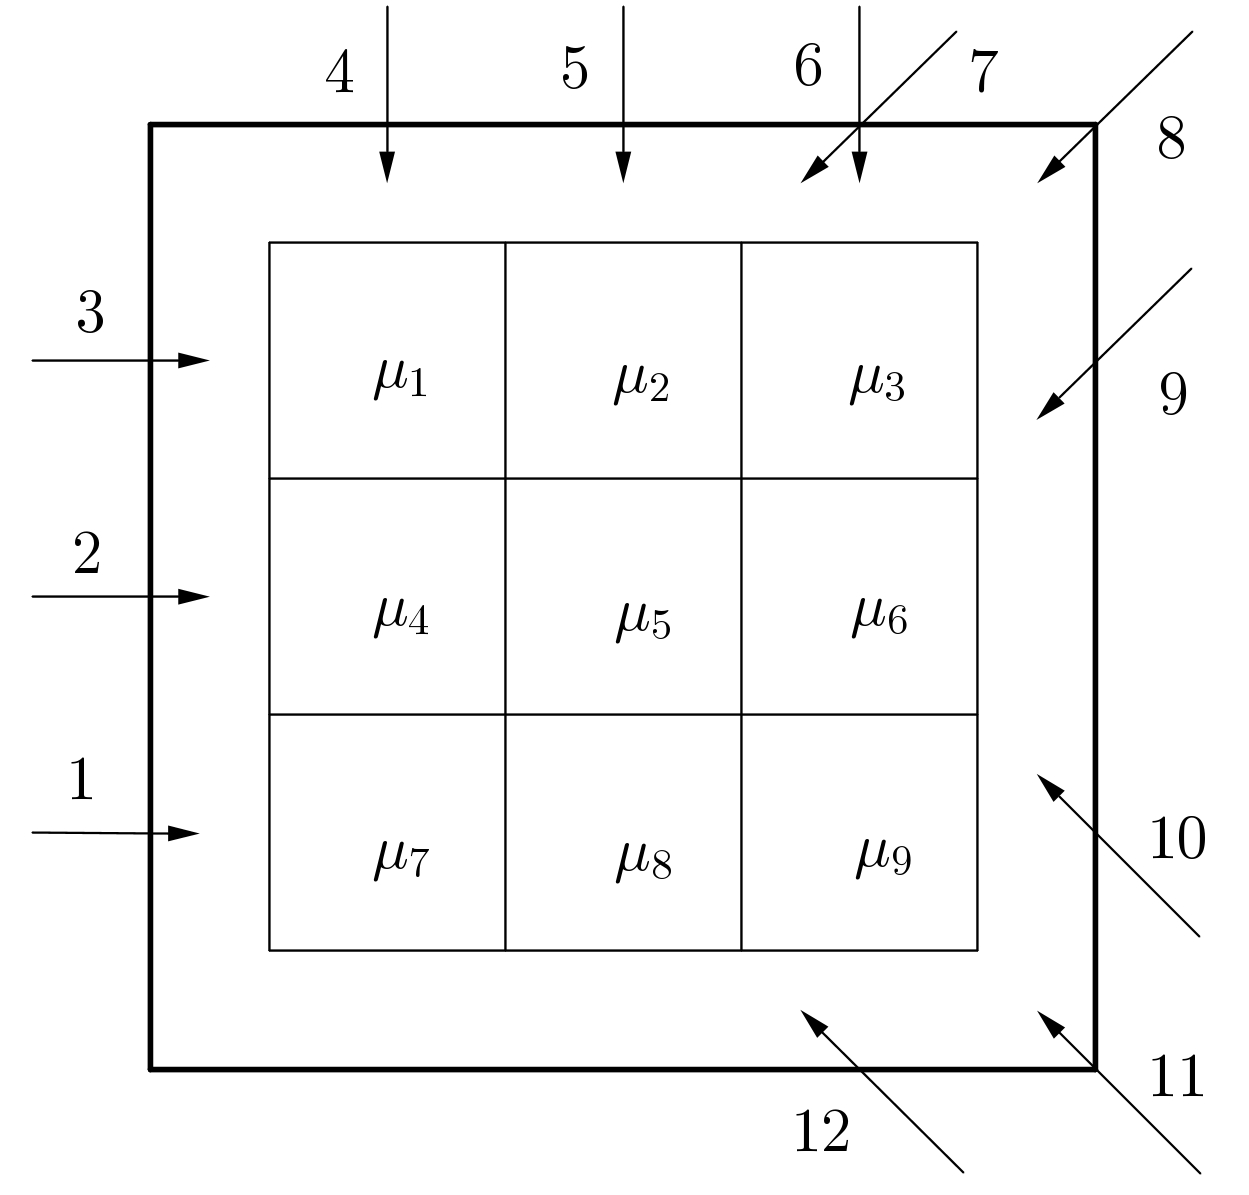
\includegraphics[scale=0.18]{../skript/domi.jpg}
\caption{Schematische Darstellung der mittleren Würfelebene sowie des umgebenden 
Aluminiummantels.}
\label{fig:Wuerfel}
\end{figure}

Vor Beginn der Messung wird die Ebene wie in Abbildung \ref{fig:Wuerfel} in neun Elementarwürfel 
der Kantenlänge $d=1$ cm eingeteilt und die Projektionsrichtungen $1,2,\ldots,12$ werden 
entsprechend gewählt. Später wird für die $i$-te Projektionen der Ausdruck $\sum_{j=1}^9 
d_{ij}\mu_j$  relevant, wobei $d_{ij}$ der Laufweg der $i$-ten Projektion durch den $j$-ten 
Elementarwürfel ist. Diese Terme können einfach durch die Schreibweise $d A\vec{\mu}$ 
zusammengefasst werden, wobei $\vec{\mu}:=(\mu_1,\ldots,\mu_9)^\text{T}$ und 
\begin{equation}
A=
\begin{pmatrix}
0	&0	&0	&0	&0	&0	&1	&1	&1	\\
0	&0	&0	&1	&1	&1	&0	&0	&0	\\
1	&1	&1	&0	&0	&0	&0	&0	&0	\\
1	&0	&0	&1	&0	&0	&1	&0	&0	\\
0	&1	&0	&0	&1	&0	&0	&1	&0	\\
0	&0	&1	&0	&0	&1	&0	&0	&1	\\
0	&\sqrt{2}	&0	&\sqrt{2}	&0	&0	&0	&0	&0	\\
0	&0	&\sqrt{2}	&0	&\sqrt{2}	&0	&\sqrt{2}	&0	&0	\\
0	&0	&0	&0	&0	&\sqrt{2}	&0	&\sqrt{2}	&0	\\
0	&\sqrt{2}	&0	&0	&0	&\sqrt{2}	&0	&0	&0	\\
s	&0	&0	&0	&\sqrt{2}	&0	&0	&0	&\sqrt{2}	\\
0	&0	&0	&\sqrt{2}	&0	&0	&0	&\sqrt{2}	&0	
\end{pmatrix} \quad . \label{eq:Matrix}
\end{equation}
Das Cäsium-Präparat wird eingesetzt und der zu vermessene Würfel in den Strahlengang gebracht. 
Die Messung geschieht mit Hilfe der Software "`winTMCA32"', welche die Daten des 
Multichannelanalyzer zu einem Channel-Counts Spektrum zusammenfasst. Die Spektren und die 
dazugehörigen um die Detektor-Totzeit korrigierten Messzeiten werden 
gespeichert.\\
Folgende Messungen werden durchgeführt:
\begin{enumerate}
\item Eine Messung ohne Würfel.
\item Von dem Würfel 0 werden die Projektionen 2,8 und 9 gemessen.
\item Von den Würfeln 1,2 und 3 werden alle Projektionen vermessen.
\end{enumerate}
Der relevante Peak im Spektrum, welcher in der Auswertung benutzt wird, liegt zwischen den 
Kanälen 257 und 315. Da eine relative Unsicherheit von maximal $0.03$ (bzw. $0.01$ bei Würfel 3) 
erwünscht ist, muss darauf geachtet werden, dass im relevanten Bereich mindestens 1200 (bzw. 
10000) Counts gemessen werden. 